\documentclass[a4paper,11pt]{article}
\usepackage[margin=2.3cm]{geometry}
\linespread{1.1}

\usepackage[T1]{fontenc}
\usepackage[utf8]{inputenc}
\usepackage[swedish]{babel}

% \usepackage{fontspec}
% \setmainfont{Linux Libertine O}

\usepackage{listings}
\usepackage{amsmath}
\usepackage{amsfonts}
\usepackage{tikz}
\usepackage{lmodern}
\usepackage{pbox}
\usepackage{fancyhdr}
\pagestyle{fancy}
\renewcommand{\headrulewidth}{ 1.0pt }
\renewcommand{\footrulewidth}{ 0.4pt }
\fancyhead{} % clear all headers
\fancyfoot{} % clear all footers

% E:even page, O:odd page, L:left, C:center, R:right
%\fancyhead[LE,RO]{\thepage}
%\fancyfoot[C]{Albert Einstein, 2009}

\fancyhead[L]{DD1350 HT15 Laboration 2}
\fancyhead[R]{Mikael Forsberg, Robin Gunning}
\fancyfoot[C]{\thepage}

\lstset{
    basicstyle=\footnotesize\ttfamily,
    breaklines=true,
    xleftmargin=0.6cm,
    showstringspaces=false,
    frame=none,
    numbers=left,
    language=Java,
    inputencoding=utf8,
    extendedchars=true,
    literate={≤}{{$\leq$}}1
}

\newcommand{\predrow}[3]{
    \pbox[t]{20cm}{\texttt{#1}} & \pbox[t]{20cm}{\texttt{#2}\\ \raisebox{-0.1cm}{\pbox[t]{20cm}{#3}} \vspace{0.33cm}}\\ 
}

\begin{document}
\pagenumbering{gobble}
\title{Laboration 2\\ Modellprovning för CTL\\ \vspace{0.2cm} \small Kungliga Tekniska Högskolan\\ Logik för dataloger\\ DD1350, HT2015}
\author{Mikael Forsberg <miforsb@kth.se>, Robin Gunning <rgunning@kth.se>}
\maketitle
\newpage

\tableofcontents
\newpage

\pagenumbering{arabic}
\section{Inledning}
Denna laboration gick ut på att implementera ett program för automatisk
modellprovning av system beskrivna med en begränsad variant av CTL i
programspråket Prolog.

\section{Metod}
I detta avsnitt presenteras den algoritm som utformades för att
utföra modellprovning, och som sedan implementerades i Prolog.

\subsection{Algoritm - informell beskrivning}
Första stycket i testerna innehåller transitionsrelationer där 
varje rad innehåller ett tillstånd och dess transitionsrelaterade tillstånd.
Sedan kommer ett stycke med sanningstilldelningar där varje rad 
innehåller en sanning för ett specifikt tillstånd. 
Tredje stycket anger i vilket tillstånd nästkommande CTL-formel ska
undersökas.
Fjärde stycket anger till sist den CTL-formel som skall kontrolleras.

\bigskip
\noindent
Vår algoritm arbetar sig igenom formeln som ett syntaxträd utifrån och in:

\begin{quote}
\texttt{ag(ef(and(x, y))) -> ag(}$\Phi_1$\texttt{)} där $\Phi_1$ \texttt{= ef(and(x, y)) -> ef(}$\Phi_2$\texttt{)} där $\Phi_2$ = \texttt{and(x, y)} ...
\end{quote}

\bigskip
\noindent
Med ovanstående i åtanke implementerar vi de olika CTL-reglerna var och en med
avseende på någon formel $\Phi$ med start i något godtyckligt tillstånd. Varje regelhanterare
tar även in listan över transitionsrelationer, listan över sanningstilldelningar samt
en lista över tidigare besökta noder.
För att
testa en given formel på ett system testar anropar vi den CTL-regel som 
hanterar den yttersta regeln (AG i ovanstående exempel) med start från det angivna
starttillståndet ur testfilens tredje stycke och den inre formeln ($\Phi_1$ i ovanstående
exempel) som argument. De flesta CTL-regelhanterare anropar sedan vidare rekursivt
till andra CTL-regler med den inre formeln som utgångspunkt. I det ovanstående exemplet skulle
regelhanteraren för EF anropats med det aktuella tillståndet och $\Phi_2$ som argument, 
följt av att regelhanteraren för AG anropats på samtliga till starttillståndet efterföljande
tillstånd med $\Phi_1$ som argument. Två regelhanterare terminerar
utan rekursion och fungerar således som basfall. Dessa två är hanteraren för en ensam
atom $p$ samt negationen av en ensam atom $\lnot p$. För de CTL-regler där det är lämpligt
läggs det aktuella tillståndet in i listan över besökta tillstånd innan listan skickas
vidare i rekursiva anrop. I andra fall görs rekursiva anrop med en tom lista för besökta
noder. Varje regelhanterare kontrollerar att den hanterade regeln tillämpats korrekt genom
att exempelvis med hjälp av listan för sanningstilldelningar verifiera att en viss sanning
gäller i det aktuella tillståndet.

\bigskip
\noindent
Med Prolog visade sig detta vara oerhört enkelt att implementera, och alla CTL-regler som
skulle användas blir väldigt naturliga att skriva som predikat, särskilt de
regler som har två fall. Vi drar även full nytta av Prologs inbyggda backtracking för att
exempelvis täcka de regler som endast kräver existens längs någon väg, samt de regler
som har flera fall.

\section{Resultat}
\noindent
Programmet klarade samtliga 730(!) testfall som anvisades i laborationslydelsen, samt våra egna två testfall (se bilagor).

\section{Predikatdokumentation}
\begin{tabular}{r l}
\textbf{Predikat} & \textbf{Beskrivning}\\
\predrow{contains/3}{contains(+List, +Key, +Value)}{Kontrollerar om värdet Value finns i den närhetslista som finns i listan av\\ närhetslistor List på index Key. Sant om värdet finns i denna närhetslista,\\ falskt i annat fall.}
\predrow{verify/1}{verify(+Filename)}{Sant om filen Filename innehåller en korrekt systembeskrivning tillsammans\\ med ett temporallogiskt påstående i begränsad CTL som gäller för systemet.\\ Falskt i annat fall.}
\predrow{validate/5}{validate(+Nodes, +Truths, +Position, +Visited, +Statement)}{Sant om det temporallogiska påståendet Statement gäller, sett från noden Start,\\ i det system som definieras av listan av närhetslistor Nodes och listan över\\ sanningstillstånd Truths. Falskt i annat fall.}
\predrow{validate\_all/5}{validate\_all(+Nodes, +Truths, +NodeList, +Visited, +Statement)}{Sant om det temporallogiska påståendet Statement gäller, sett från \textbf{samtliga}\\ noder ur NodeList, i det system som definieras av listan av närhetslistor Nodes\\ och listan över sanningstillstånd Truths. Falskt i annat fall.}
\predrow{validate\_one/5}{validate\_one(+Nodes, +Truths, +NodeList, +Visited, +Statement)}{Sant om det temporallogiska påståendet Statement gäller, sett från \textbf{någon} nod\\ ur NodeList, i det system som definieras av listan av närhetslistor Nodes och\\ listan över sanningstillstånd Truths. Falskt i annat fall.}

\end{tabular}

\newpage
\section{Bilagor}
\subsection{Eget system: ett nätforum}
\begin{itemize}
\item[] \emph{u} : Autentiserad användare
\item[] \emph{a} : Autentiserad administrator
\item[] \emph{p} : Postar meddelande
\item[] \emph{d} : Raderar ett eller flera meddelanden
\end{itemize}

\bigskip

\noindent
Egenskap som gäller:
\begin{quote}
Testfil: se bilaga ''egetsys-valid.txt''
\end{quote}
\begin{quote}
\emph{Det går alltid att nå ett tillstånd där man som inloggad användare
kan posta meddelanden.}
\end{quote}
$$
{\cal M}_{\mathrm{Start}} \models \mathrm{AG}\:\mathrm{EF} (u \land p)
$$

\vspace{0.5cm}

\noindent
Egenskap som inte gäller: (eftersom administrator även räknas som användare)
\begin{quote}
Testfil: se bilaga ''egetsys-invalid.txt''
\end{quote}
\begin{quote}
\emph{Det gäller alltid att vanliga användare inte kan radera poster.}
\end{quote}
$$
{\cal M}_{\mathrm{Start}} \models \mathrm{AG} (\lnot d \lor \lnot u)
$$

\vspace{0.5cm}

% s0 = Start
% s1 = Logged in (user)
% s2 = Post_1
% s3 = Logged in (admin)
% s4 = Delete
% s5 = Post_2

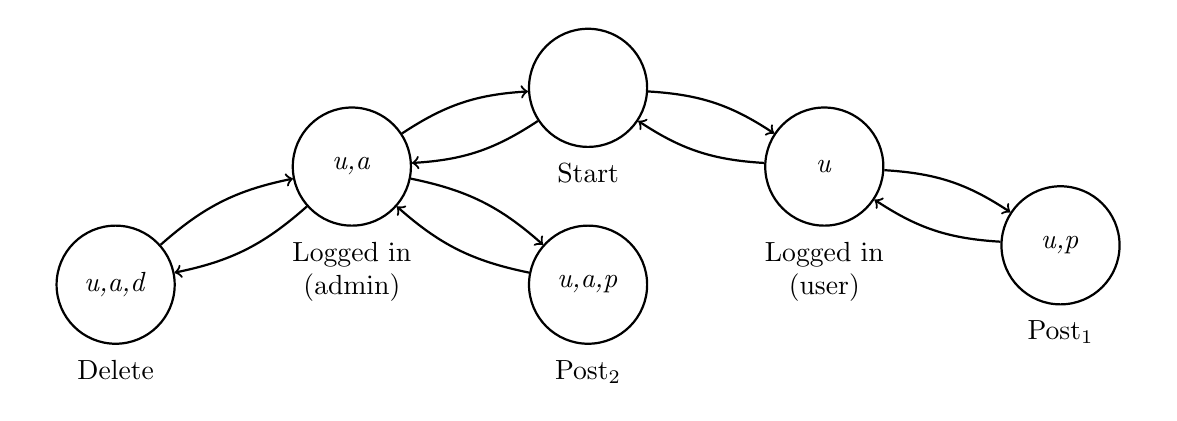
\begin{tikzpicture}
\node[label={[text width=2cm, align=center, below=1.6cm]Start},draw, thick, circle, minimum size=1.5cm] (start) at (0, 0) {};
\node[label={[text width=2cm, align=center, below=1.6cm]Logged in\\ (user)}, draw, thick, circle, minimum size=1.5cm] (authuser) at (3, -1) {\emph{u}};
\node[label={[text width=2cm, align=center, below=1.6cm]Post\textsubscript{1}}, draw, thick, circle, minimum size=1.5cm] (userpost) at (6, -2) {\emph{u,p}};

\node[label={[text width=2cm, align=center, below=1.6cm]Logged in\\ (admin)}, draw, thick, circle, minimum size=1.5cm] (authadmin) at (-3, -1) {\emph{u,a}};
\node[label={[text width=2cm, align=center, below=1.6cm]Post\textsubscript{2}}, draw, thick, circle, minimum size=1.5cm] (adminpost) at (0, -2.5) {\emph{u,a,p}};
\node[label={[text width=2cm, align=center, below=1.6cm]Delete}, draw, thick, circle, minimum size=1.5cm] (admindel) at (-6, -2.5) {\emph{u,a,d}};
% \draw (start) edge[out=12,in=110,->] (authuser);
% \draw[->] (start) to [out = 25, in = 90, looseness = 0.5] (authuser);
\draw[thick,->] (start) to [bend left=15] (authuser);
\draw[thick,->] (authuser) to [bend left=15] (start);
\draw[thick,->] (authuser) to [bend left=15] (userpost);
\draw[thick,->] (userpost) to [bend left=15] (authuser);

\draw[thick,->] (start) to [bend left=15] (authadmin);
\draw[thick,->] (authadmin) to [bend left=15] (start);
\draw[thick,->] (authadmin) to [bend left=15] (adminpost);
\draw[thick,->] (adminpost) to [bend left=15] (authadmin);
\draw[thick,->] (authadmin) to [bend left=15] (admindel);
\draw[thick,->] (admindel) to [bend left=15] (authadmin);
\end{tikzpicture}

\newpage
\subsection{egetsys-valid.txt}
\lstinputlisting[tabsize=4]{../egetsys-valid.txt}

\newpage
\subsection{egetsys-invalid.txt}
\lstinputlisting[tabsize=4]{../egetsys-invalid.txt}

\newpage
\subsection{labb2.pl}
\lstinputlisting[tabsize=4]{../labb2.pl}


\end{document}
